%%%%%%%%%%%%%%%%%%%%%%%%%%%%%%%%%%%%%%%%%
% Simple Sectioned Essay Template
% LaTeX Template
%
% This template has been downloaded from:
% http://www.latextemplates.com
%
% Note:
% The \lipsum[#] commands throughout this template generate dummy text
% to fill the template out. These commands should all be removed when 
% writing essay content.
%
%%%%%%%%%%%%%%%%%%%%%%%%%%%%%%%%%%%%%%%%%

%----------------------------------------------------------------------------------------
%	PACKAGES AND OTHER DOCUMENT CONFIGURATIONS
%----------------------------------------------------------------------------------------

\documentclass[a4paper,12pt]{article} % Default font size is 12pt, it can be changed here

\usepackage[portuguese]{babel}
\usepackage{natbib}
\usepackage{url}
\usepackage[utf8x]{inputenc}
\usepackage{amsmath}
\usepackage{parskip}
\usepackage{fancyhdr}
%\usepackage{vmargin}
\usepackage{amsmath,amsthm,amssymb,caption}
\usepackage{cite}
\usepackage{epsfig}
\usepackage[T1]{fontenc}
\usepackage{times,mathptmx}
\usepackage{float}
\usepackage{color}
\usepackage{listings}
\usepackage{fancyhdr}

\usepackage{geometry} % Required to change the page size to A4
\geometry{a4paper} % Set the page size to be A4 as opposed to the default US Letter

\usepackage{graphicx} % Required for including pictures

\usepackage{float} % Allows putting an [H] in \begin{figure} to specify the exact location of the figure
\usepackage{wrapfig} % Allows in-line images such as the example fish picture

\usepackage{lipsum} % Used for inserting dummy 'Lorem ipsum' text into the template

%% ------- Watermark -------
\usepackage{draftwatermark}
\SetWatermarkText{
\includegraphics{minerva_watermark}}
\SetWatermarkAngle{0}
\SetWatermarkLightness{1}
\SetWatermarkScale{0.9}

\linespread{1.2} % Line spacing

\lstdefinestyle{customc}{
	belowcaptionskip=1\baselineskip,
	breaklines=true,
	%%frame=L,
	xleftmargin=\parindent,
	language=C,
	showstringspaces=false,
	basicstyle=\footnotesize\ttfamily,
	keywordstyle=\bfseries\color{green!40!black},
	commentstyle=\itshape\color{purple!40!black},
	identifierstyle=\color{blue},
	stringstyle=\color{orange},
}

\lstdefinestyle{customasm}{
	belowcaptionskip=1\baselineskip,
	frame=L,
	xleftmargin=\parindent,
	language=[x86masm]Assembler,
	basicstyle=\footnotesize\ttfamily,
	commentstyle=\itshape\color{purple!40!black},
}

\lstset{escapechar=@,style=customc}

%\setlength\parindent{0pt} % Uncomment to remove all indentation from paragraphs

\graphicspath{{Pictures/}} % Specifies the directory where pictures are stored

\begin{document}

\fancypagestyle{plain}{%
	\fancyhf{} % clear all header and footer fields
	\fancyfoot[L]{
\includegraphics[width=7cm]{minerva-color}}
	\renewcommand{\headrulewidth}{0pt}
	\renewcommand{\footrulewidth}{0pt}}

%----------------------------------------------------------------------------------------
%	TITLE PAGE
%----------------------------------------------------------------------------------------

\begin{titlepage}
\thispagestyle{plain}
\newcommand{\HRule}{\rule{\linewidth}{0.5mm}} % Defines a new command for the horizontal lines, change thickness here

\center % Center everything on the page

\textsc{\LARGE Universidade Federal do Rio de Janeiro}\\[1.5cm] % Name of your university/college
\textsc{\Large Circuitos Elétricos II}\\[0.5cm] % Major heading such as course name
\textsc{\large Professor Antônio Carlos Moreirão de Queiroz}\\[0.5cm] % Minor heading such as course title

\HRule \\[0.4cm]
{ \huge \bfseries Análise Nodal Modificada
	Para Circuitos Lineares com Transistores MOS: Ponto de Operação e Resposta em Frequência}\\[0.4cm] % Title of your document
\HRule \\[1.5cm]
\vspace*{5cm}
\hspace*{10cm}
\begin{minipage}{0.4\textwidth}
\begin{flushleft} \large
\emph{Alunos:}\\
Joao Pedro K. Marques\\Maria Luiza C. Vianna\\Miguel de Sousa\\ % Your name
\end{flushleft}
\end{minipage}
~



\end{titlepage}

%	INTRODUCTION
%----------------------------------------------------------------------------------------
\section{Introdução}
Como trabalho da matéria de Circuitos Elétricos II, o nosso grupo desenvolveu o simulador OrKappes (trocadilho entre o nome do nosso membro e o famoso programa simulador de circuitos). O programa resolve por meio do método da Análise Nodal Modificada circuitos lineares que comportam os seguintes elementos: Resistor, Indutor, Acoplamento entre Indutores, Capacitor, Fonte de tensão controlada a tensão, Fonte de corrente controlada a corrente, Fonte de corrente controlada a tensão, Fonte de tensão controlada a corrente, Fonte de corrente, Fonte de tensão, Amplificador Operacional Ideal e o Transistor MOS(tanto canal N como canal P).\\ 
Desenvolvemos o programa em C++ com o VisualStudios 2015 e utilizamos a plataforma GitHub como controle de versão. Escolhemos C++ pela facilidade da orientação a objeto e escolhemos o GitHub pois é uma das ferramentas mais utilizadas hoje em dia para controle de versão.

\section{OrKappes}
%----------------------------------------------------------------------------------------
\subsection{Funcionamento} % Sub-section
 O programa principal lê um arquivo do tipo ".net" que contém a netlist a ser processada. Após, ele cria objetos para cada componente de forma dinâmica, isso garante que o nosso programa não tenha um número limite de componentes. A partir da criação do array de componentes, é a hora de montar as suas estampas na matriz de ponto de operação ( GMatrix ) e processá-la com o algorítmo de Newton-Raphson, caso haja algum componente a ser linearizado. Com a matriz de condutância pronta, utilizamos um resolvedor de sistemas lineares que utiliza o Método de Gauss-Jordan com condensação pivotal para nos informar as tensões e correntes do sistema: o ponto de operação. Vale um comentário a respeito do MOSFET, como ele é um objeto, a cada iteração do Newton-Raphson os parâmetros dele são calculados, até suas capacitâncias parasitas. Isso evita que precisemos calculá-las na hora de realizar a análise espectral.\\ 
 Depois de calcular o ponto de operação, as tensões e correntes são salvas em arquivos ".dc" e o programa começa a fazer a análise da resposta em frequência. Nessa parte, montamos a matriz de condutância AC e varremos o sistema desde a frequência mais baixa até a mais alta, variando o passo de acordo com o informado pela netlist. Ao final dessa etapa, o programa salva a solução para cada frequência em um arquivo ".tab".
 \subsection{Métodos do Programa}
 \subsubsection{Netlist(string netlistPath)}
 Função recebe o path para o arquivo ".net", lê a net list e armazena o array de componentes. Nesse método calcula-se o número de tensões e de correntes do sistema.
  \subsubsection{DoConductanceMatrixDC(void)}
  Utiliza o array de componentes da classe Netlist e compõe a matriz de condutancia, essa matriz é gerada dinamicamete a partir do numero de tensões e de correntes do sistema.
  \subsubsection{NewtonRaphson(void)}
  Nesse método, é implementado o conhecido algorítmo de Newton-Raphson.
  \subsubsection{WriteDCData(void)}
  Salvamos o ponto de operação em um arquivo ".dc".
  \subsubsection{ACSweep(void)}
  Montamos as estampas AC e resolvemos para cada frequência o sistema linear complexo por meio do Método de Gauss-Jordan com condensação pivotal. Por fim, guardamos o resultado em um arquivo ".tab"
 \subsection{Exemplos}
  \subsubsection{LeapFrog:}
  \begin{itemize}
  	\item Netlist
  	\begin{lstlisting}
  	15
  	R0100 1 0 1E+3
  	R0203 2 3 1E+3
  	R0402 4 2 1E+3
  	R0504 5 4 1E+3
  	R0105 1 5 1E+3
  	R0603 6 3 1E+3
  	R0701 7 1 1E+3
  	R0809 8 9 1E+3
  	R1011 10 11 1E+3
  	R1208 12 8 1E+3
  	R1310 13 10 1E+3
  	R0614 6 14 1E+3
  	R1206 12 6 1E+3
  	R1512 15 12 1E+3
  	R1315 13 15 1E+3
  	R0713 7 13 1E+3
  	C0902 9 2 9.32778700555236E-7
  	C1105 11 5 1.4031540561078E-6
  	C1503 15 3 1.7274276550171E-6
  	C0115 1 15 5.79956913281569E-7
  	C0603 6 3 3.97974815527259E-6
  	C1504 15 4 5.69845860607148E-6
  	C0701 7 1 3.51512140879876E-6
  	C0406 4 6 1.7274276550171E-6
  	C0704 7 4 5.79956913281569E-7
  	O0900 9 0 2 0
  	O1100 11 0 5 0
  	O0300 3 0 6 0
  	O0400 4 0 15 0
  	O0100 1 0 7 0
  	O1200 12 0 8 0
  	O1300 13 0 10 0
  	V1400 14 0 1
  	.AC DEC 2 0.1 1000
  	\end{lstlisting}
  	\item Resultado:
  	\begin{figure}[h!]
\centering
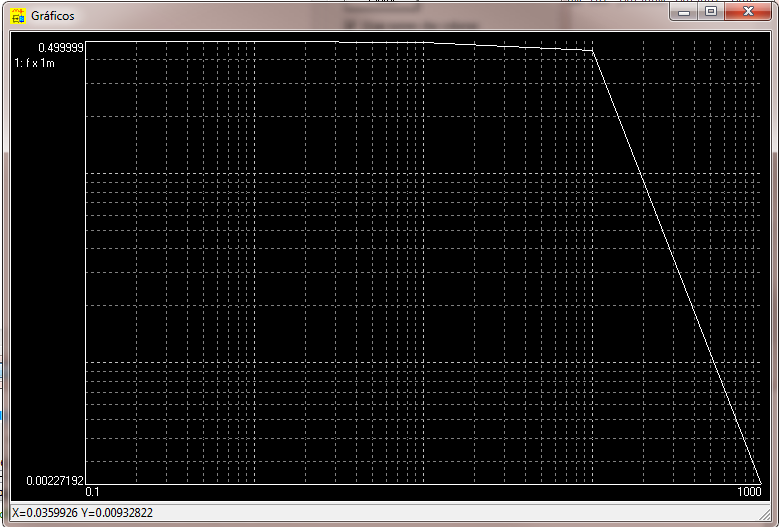
\includegraphics[width=1\linewidth]{leapfrog}

\label{Gráfico LeapFrog}
\end{figure}

  \end{itemize}
%----------------------------------------------------------------------------------------


\end{document}